\documentclass[UTF-8,10.5pt]{ctexart}
\usepackage{geometry}
\usepackage{graphicx}
\usepackage[namelimits]{amsmath} %数学公式
\usepackage{amssymb}             %数学公式             %数学字体
\usepackage{mathrsfs} 
\usepackage{txfonts}
\usepackage{float}  %设置图片浮动位置的宏包
\usepackage{subfigure}%插入多图时用子图显示的宏包
\usepackage{booktabs}
\usepackage{fontspec}
\setmainfont{Times New Roman}
\geometry{a4paper,scale=0.85}
\author{左熙辰\thanks{北京大学生命科学学院;e-mail:m13333318502@163.com}}
\date{}
\title{麻醉剂和酒精对斑马鱼幼体的影响}
\renewcommand{\abstractname}{\normalsize 摘要\\}
\begin{document}
    \maketitle
    \begin{abstract}
        \normalsize
        斑马鱼是一种实验室常见的小型脊椎动物,因其发育过程较为简单,卵透明便于观察发育全过程而受到科学家青睐,本文将使用野生型斑马鱼探究麻醉剂和乙醇对斑马鱼幼体心率的影响。
        \paragraph*{关键字}斑马鱼\text{ }发育生物学\text{ } 心率 
    \end{abstract}
    \section{实验方法}
    1. 将含有48-72hpf 斑马鱼胚胎的小培养皿置于解剖镜下观察(使用透射光源),用大头针
轻碰胚胎,检测其是否具有触碰反应。观察其各个部分结构,找到心房和心室,随机挑选3
个胚胎检测其心率(计时30s),每个做3 次重复,记录数据

2. 用吸管吸取鱼水,加入0.16mg/ml 的Tricaine 溶液(三卡因,麻醉剂),约2min 后检测其触碰反
应,检测心率(方法同上),记录数据

3. 用吸管吸走培养皿中的溶液,换上新鲜的鱼水,约3min 后检测其触碰反应,检测心率(方
法同上),记录数据

4. 用吸管吸走鱼水,换加5\%酒精溶液,立即检测其触碰反应并快速检测心率(方法同上),
记录数据

5. 部分胚胎心率降到0 后立即吸走酒精,换上新鲜的鱼水,一段时间后检测其触碰反映,
检测心率(方法同上),记录数据
实验
\begin{figure}[htbp]
    \centering
    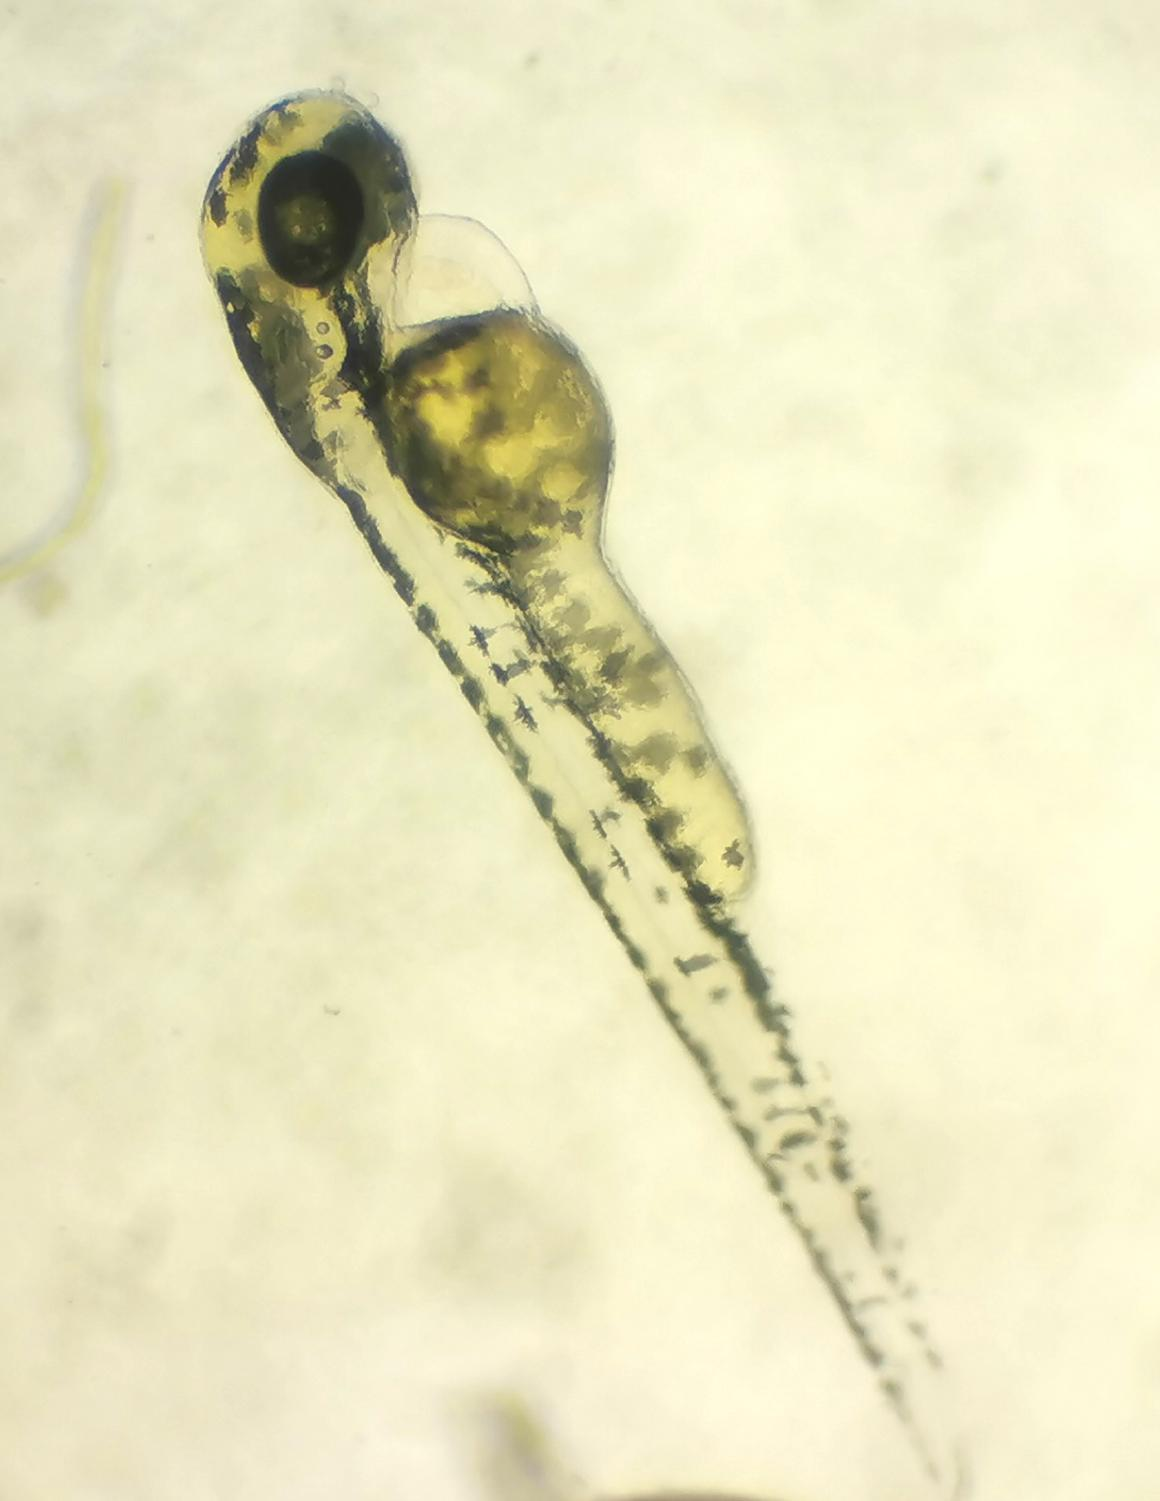
\includegraphics[scale = 0.8]{src/zoology/R2DJK5Z.jpg}
    \caption{解剖镜下斑马鱼胚胎形貌}
\end{figure}
    \section{实验结果及结论}
    实验用斑马鱼如图1。原始数据见表1。实验结果如图2所示,三卡因处理后和移除后,心率基本不变,推测是由于心源性活动并未受到抑制,导致心率没有显著变化;而三卡因移除后的心率上升,推测是由于测试触碰反应时斑马鱼的应激反应导致心率升高,而乙醇处理后,心率活动受到一定的抑制但结果并不显著,推测是心肌细胞受到乙醇毒害但作用时间较短使得损害效果不明显,乙醇移除后,心率逐步恢复。
    乙醇处理组斑马鱼胚胎的表现值得注意:胚胎在酒精溶液中痛苦剧烈地扭动,对触碰的反应也非常剧烈,测量心率时,胚胎的心率逐渐降低。

    \begin{figure}[htbp]
        \label{fig1}
        \centering
        \subfigure[]{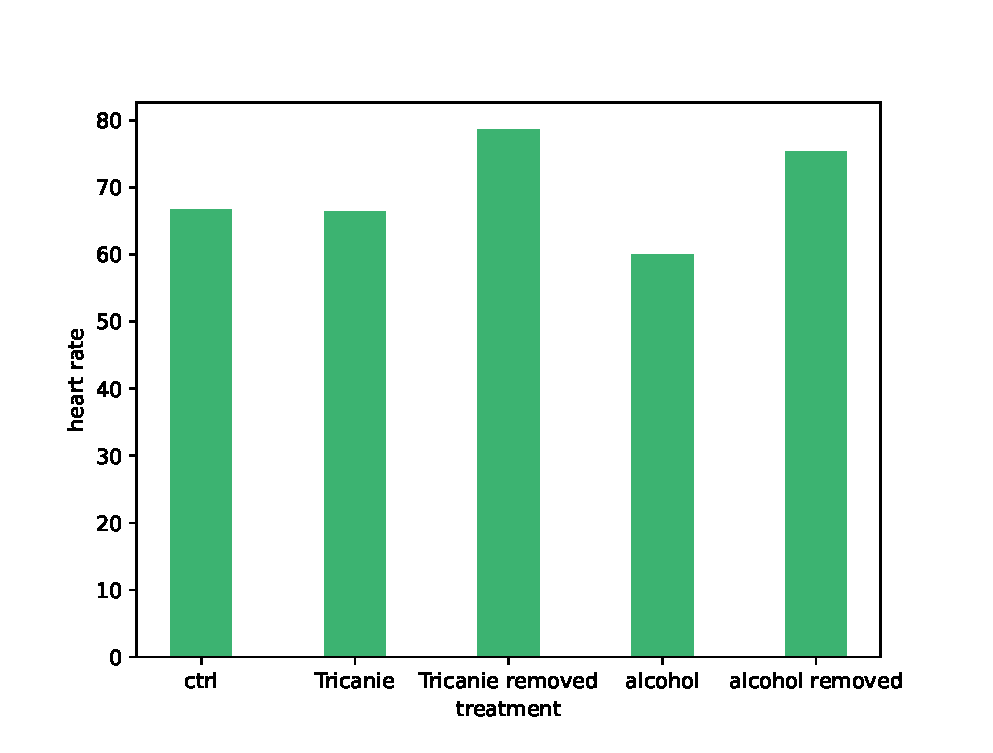
\includegraphics[scale = 0.5]{src/zoology/Figure1.eps}}
        \subfigure[]{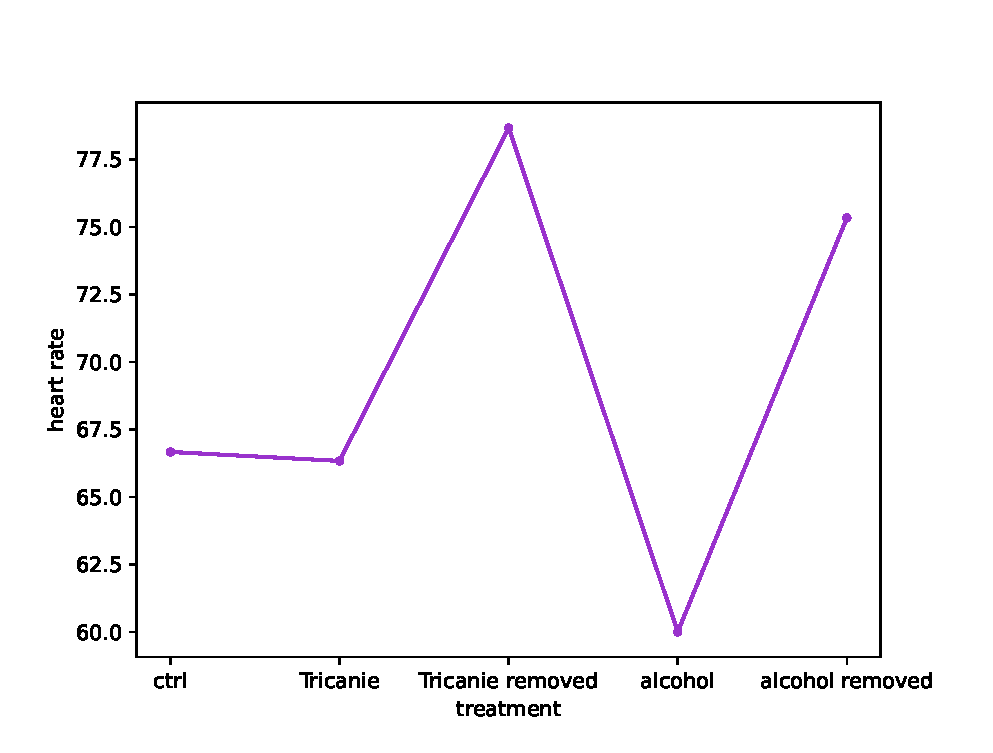
\includegraphics[scale = 0.5]{src/zoology/Figure2.eps}}
        \caption[]{\textbf{不同处理对斑马鱼幼体心率的影响.}其中ctrl为处理前对照,Tricanie为三卡因处理组,Tricanie removed为三卡因移除组,
        Alcohol为乙醇处理组,Alchol removed为乙醇移除组,ctrl组与Tricaine组采用Student's-t检验,剩下相邻两组进行Kolmogorov-Smirnov检验,五组中,除Alcohol处理组有不显著下降以及Tricaine removed组和Alcohol removed组有不显著回升外其余均无显著差异(\textit{P}=0.91, 0.09, 0.09, 0.6, 0.6; \textit{P}>0.05)}
    \end{figure}
    % Please add the following required packages to your document preamble:
% \usepackage{booktabs}
\begin{center}
\begin{table}[hp]
    \centering
    \label{table}
    \caption{斑马鱼不同处理下的心率}
    \begin{tabular}{@{}cccccc@{}}
    \toprule
        & Ctrl & Tricaine & Tricaine removed & Alcohol & Alcohol removed \\ \midrule
    第一次 & 63   & 67      & 82              & 80      & 78              \\
    第二次 & 67   & 70      & 77              & 50      & 70              \\
    第三次 & 70   & 62      & 77              & 50      & 78              \\ \bottomrule
    \end{tabular}
    \end{table}
\end{center}
    \section{致谢}
    感谢董巍、李大建老师和高远助教在实验过程中的大力支持!感谢所有无私提供实验数据的同学!
\end{document}